\documentclass[../main.tex]{subfiles}

\begin{document}
\chapter{Designing and Implementing the Graphics Library} \label{ch:graphics}
    The graphics library is a key component of the system, as it provides the
        functionality for creating images and animations using Haskell.
    The implementation of the graphics library is largely independent of the rest
        of the system.
    It is responsible for generating the necessary data to render images and
        animations, rather than rendering them itself.
    The website is responsible for rendering the images and animations at the
        correct frame rate, using the data generated by the graphics library.

    Throughout this chapter, there are several code snippets, which are taken from
        the implementation of the graphics library.
    In most cases, the implementations are trivial, so have been omitted for
        brevity, and in some cases, verbose type signatures have been replaced with
        ellipses.
    The full implementation of the graphics library can be found in
        Appendix~\ref{app:code}.

    \section{Library Overview}
        There were several sources of inspiration for the graphics library, including
            CodeWorld and P5.js.
        P5.js, a JavaScript library, is inherently imperative, relying heavily on side
            effects and global state.
        Despite that, P5.js provides a straightforward API, with a nice selection of
            well-named functions, many of which can be adapted to fit the functional
            programming paradigm.
        CodeWorld, on the other hand, uses Haskell, so it is purely functional, with no
            side effects or global state, relying instead on function composition and
            recursion.
        While CodeWorld's API provides an excellent example of a functional graphics
            library, it is less straightforward than P5.js.
        The aim for our library is to find a balance between the simplicity of P5.js,
            and the functional design of CodeWorld.

        \subsection{Required Modules}
            We need to consider what a graphics library needs to be able to do, from the
                perspective of a user.
            \begin{itemize}
                \item Represent the two-dimensional space to draw on, i.e. the canvas.
                \item Represent the graphical primitives that can be drawn in that space, i.e.
                      shapes.
                \item Apply transformations and colours to these shapes.
                \item Generate the data to allow the website to render the image or animation.
            \end{itemize}

            The graphics library is split into six modules:
            \begin{itemize}
                \item \texttt{Lib} — the main module, which exports the public API for the library.
                      This has one function, \texttt{render}, which takes a \texttt{Canvas} and
                          prints its JSON representation to the standard output.
                      It is the responsibility of the website to render this as an image or
                          animation.
                      This function makes use of Haskell's \texttt{IO} monad, which allows for side
                          effects, such as printing to the standard output.

                      \begin{lstlisting}[language={Haskell}, label={lst:lib}, caption={The 
                        \texttt{render} function.
                        The \texttt{IO ()} return type means that the function has side effects, 
                        specifically printing to the standard output, but no value is returned.}]
render :: Canvas -> IO ()\end{lstlisting}

                \item \texttt{Internal} — an internal module, which contains the types and
                      functions used by the library, which are not exposed to the user.
                      This includes the functions to convert each type to their JSON representation.

                \item \texttt{Canvas} — the module for creating and modifying the canvas.

                \item \texttt{Shape} — the module for creating and modifying graphical primitives.

                \item \texttt{Maths} — the module for providing various mathematical functions and
                      types, such as vectors and angles.

                \item \texttt{Color} — the module for providing several representations for colours.
            \end{itemize}

            The following sections will provide an overview of these last four modules.
            As the \texttt{Color} and \texttt{Maths} modules are the simplest, and are
                required by the \texttt{Shape} and \texttt{Canvas} modules, we will work from
                the bottom up, starting with the \texttt{Color} module.

    \section{The \texttt{Color}
        Module} The \texttt{Color} module is the simplest of the four modules, as it
            only needs to provide a way to represent colours.

        \subsection{Common Digital Colour Representations}
            There are several ways to represent colours in a graphics library, each with
                its own advantages and disadvantages.
            Some common representations are hexadecimal, RGB, HSL and HSV.

            \subsubsection{RGB and Hexadecimal}
                The hexadecimal and RGB (red, green, blue) representations are two ways of
                    representing the same thing, with the former being more concise, and the latter
                    more readable.
                They both represent the colour as a combination of red, green and blue, with
                    each component being an integer between 0 and 255, so are naturally suited to
                    digital displays, which use red, green and blue light to create colours.

                The RGB representation uses a tuple of three base ten integers to represent the
                    red, green and blue components, respectively.
                This tuple is commonly written as a comma-separated list of integers, enclosed
                    in parentheses, prefixed by the \texttt{RGB} constructor, e.g. \texttt{RGB(255,
                        0, 0)} for red.

                Hexadecimal colours combine the red, green and blue components into a single
                    base sixteen number.
                This is written as a string, starting with a hash symbol, followed by three
                    pairs of hexadecimal digits, representing the red, green and blue components,
                    respectively, e.g. \texttt{"\#FF0000"} for red.

                These representations can be visualised as a cube, with the x, y and z axes
                    representing the red, green and blue components, respectively, as shown in
                    Figure~\ref{fig:rgb}.

                \begin{figure}[H]
                    \centering
                    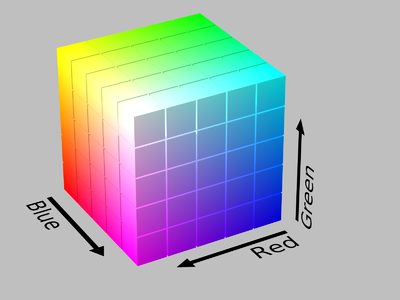
\includegraphics[width=0.45\linewidth]{rgb.png}
                        \caption{The RGB colour space.
                            Image taken from \href{https://en.wikipedia.org/wiki/HSL_and_HSV}{Wikipedia:
                                    HSL and HSV}.
                        }
                        \label{fig:rgb}
                \end{figure}

                Both RGB and hexadecimal colours can be extended to support an alpha channel,
                    allowing for transparency.
                For RGBA, the alpha channel is represented as a floating point number between
                    0.0 and 1.0, with 0.0 being fully transparent, and 1.0 being fully opaque.
                The alpha channel in hexadecimal colours is represented as a pair of
                    hexadecimal digits, with 00 being fully transparent, and FF being fully opaque.

            \subsubsection{HSL and HSV}
                HSL and HSV are almost identical representations, with HSL representing the
                    colour as a hue, saturation and lightness, and HSV (also known as HSB)
                    representing the colour as a hue, saturation and value (or brightness).
                These representations are visualised as a cylinder, with the hue, saturation
                    and lightness/value components representing the angle, radius and height,
                    respectively, as shown in Figure~\ref{fig:hsl}.

                \begin{figure}[H]
                    \centering
                    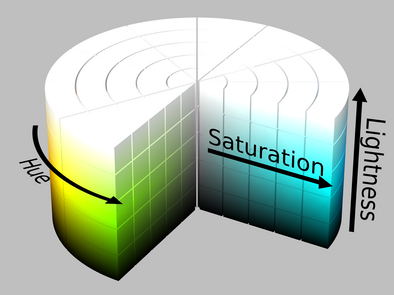
\includegraphics[width=0.45\linewidth]{hsl.png}
                    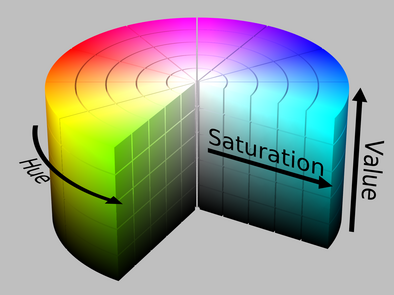
\includegraphics[width=0.45\linewidth]{hsv.png}
                        \caption{The HSL and HSV colour spaces.
                            Images taken from \href{https://en.wikipedia.org/wiki/HSL_and_HSV}{Wikipedia:
                                    HSL and HSV}.
                        }
                        \label{fig:hsl}
                \end{figure}

                The hue component is an angle between 0 and 360 degrees, with 0 and 360
                    representing red, 120 representing green, 240 representing blue.
                The saturation component is a percentage between 0\% and 100\%, with 0\%
                    representing a shade of grey, and 100\% representing a fully saturated colour.
                The lightness/value component is also a percentage between 0\% and 100\%.
                For HSL, 0\% represents black, 100\% represents white, and 50\% represents the
                    colour itself.
                For HSV, 0\% represents black, 100\% represents the colour itself, and 50\%
                    represents white.

                As with RGB and hexadecimal colours, HSL and HSV can also be extended to
                    support an alpha channel, with the alpha channel being represented in the same
                    way as for RGBA colours.

        \subsection{The Color Type}
            For the purposes of this library, it made sense to consider what other
                libraries used for colour representation.
            CodeWorld offered both RGB and HSL, as well as a limited selection of named
                colours.
            Meanwhile, P5.js, as a JavaScript library, used any representation supported by
                CSS.
            Given that this library is designed to be used in a web browser, it made sense
                to follow P5.js' lead, and support all the colour representations that CSS
                supports: hexadecimal, RGB, RGBA, HSL and HSLA, as well as a selection of named
                colours~\citep{cssColours}.

            As such, the \texttt{Color} type has 153 constructors.
            Named colours comprise 148 of these constructors, with the remaining five
                constructors representing the other colour representations supported by CSS.

            \begin{lstlisting}[language={Haskell}, label={lst:color}, caption={The \texttt{Color} type definition.
                Named colours have been omitted, but are included in the actual implementation, as seen 
                in Appendix~\ref{app:code}.}]
data Color
    = RGB Int Int Int -- Red, Green, Blue (0-255)
    | RGBA Int Int Int Float -- RGB + Alpha (0.0-1.0)
    | Hex String -- Hexadecimal, # optional, case insensitive
    | HSL Int Int Int -- Hue (0-360), Saturation, Lightness (0-100)
    | HSLA Int Int Int Float -- HSL + Alpha (0.0-1.0)
    | ... -- Type constructors for named colours omitted\end{lstlisting}

    \section{The \texttt{Maths}
        Module} The \texttt{Maths} module is the next simplest module, as the majority
            of the mathematical functions a user would need are provided by Haskell's
            standard library.
        However, there are a few types and functions that are not provided by the
            standard library, but are useful for a graphics library.

        \subsection{The \texttt{Length}
            Type} The first of these is the \texttt{Length} type, which is used to
                represent lengths, such as the width and height of the canvas, the radius of a
                circle, the side length of a square.
            It is simple a type alias for \texttt{Float}, so provides no additional type
                safety, but does provide a level of semantic clarity, particularly in the
                documentation.
            \begin{lstlisting}[language={Haskell}, label={lst:length}, caption={The \texttt{Length} type definition.}]
type Length = Float\end{lstlisting}

        \subsection{Angles}
            Angles are another fundamental part of any graphics library, as they are
                essential for rotations.
            There are several units for measuring angles, including degrees, radians,
                gradians and turns.
            The two most common units are degrees and radians, with degrees dividing a
                circle into 360 parts, and radians dividing a circle into $2\pi$ parts.
            Given that, it makes sense to provide users with the ability to work with both
                of these, and functions for converting between them.

            We can define two more type aliases for \texttt{Float}, \texttt{Degrees} and
                \texttt{Radians}, to provide a level of semantic clarity, as with the
                \texttt{Length} type.
            We can then define functions for converting between degrees and radians.

            \begin{lstlisting}[language={Haskell}, label={lst:angleFns}, caption={The angle functions.}]  
type Degrees = Float
type Radians = Float                
radians :: Degrees -> Radians
degrees :: Radians -> Degrees\end{lstlisting}

        \subsection{The \texttt{Vector}
            Type} Vectors are a fundamental part of any graphics library, as they can be
                used to represent points, directions, velocities, forces, etc. As this library
                works with just two dimensions, our vectors only need to have two components,
                an x and a y.
            Both P5.js and CodeWorld provide a \texttt{Vector} type, with the latter also
                providing a \texttt{Point} type, which is identical to a \texttt{Vector}.
            For simplicity, we use a single \texttt{Vector} type to represent points,
                directions, and anything else the user may need.
            The \texttt{Vector} type therefore has a single constructor with two type
                parameters, both of type \texttt{Float}.
            Note the use of the \texttt{Float} type over the \texttt{Length} type, once
                again for semantic clarity, as vectors are often used to represent several
                concepts, as mentioned above.
            An alternative to using a custom \texttt{Vector} type would be to use a tuple
                of \texttt{Float}s, but this would not provide the same level of type safety.
            For example, a function that takes a \texttt{Vector} as an argument would not
                accept a tuple of \texttt{Float}s, even though they are semantically the same.

            \begin{lstlisting}[language={Haskell}, label={lst:vector}, caption={The \texttt{Vector} type definition.}]
data Vector = Vector Float Float\end{lstlisting}

            \subsubsection{Vector Operations}
                Alongside the \texttt{Vector} type, it is useful to provide a simple set of
                    functions for working with vectors.
                These functions include addition, subtraction, scalar multiplication, scalar
                    division, dot product, magnitude, argument and normalisation.
                For the first four functions, we could make \texttt{Vector} an instance of the
                    \texttt{Num} type class, but this would require us to define all the functions
                    in \texttt{Num}, which is unnecessary, as we only need a subset of them.
                Moreover, there is no defined division or multiplication for vectors, so it
                    would be misleading to make \texttt{Vector} an instance of \texttt{Num}.
                We can instead define the operators \verb|^+^|, \verb|^-^|, \verb|^*^| and
                    \verb|^/^|.
                These names reflect the standard \verb|+|, \verb|-|, \verb|*| and \verb|/|
                    operators, but with wrapped by carets (\verb|^|) to indicate that they are for
                    vectors, based on the standard mathematical notation for vectors, which uses a
                    caret above the vector symbol.

                \begin{lstlisting}[language={Haskell}, label={lst:vectorOps}, caption={The vector operators.}]
-- Vector addition
(^+^) :: Vector -> Vector -> Vector
-- Vector subtraction
(^-^) :: Vector -> Vector -> Vector
-- Scalar multiplication
(^*^) :: Vector -> Float -> Vector
-- Scalar division
(^/^) :: Vector -> Float -> Vector\end{lstlisting}

                The remaining functions are equally simple to define, and make use of several
                    functions from the \texttt{Prelude} module.
                Note that there is no cross product function, as this is only defined for
                    three-dimensional vectors.

                \begin{lstlisting}[language={Haskell}, label={lst:vectorFns}, caption={The remaining vector functions.}]
-- Calculates the magnitude (length) of a vector
mag :: Vector -> Length
-- Calculates the argument (polar angle) of a vector
arg :: Vector -> Radians
-- Normalises a vector, i.e. returns a vector with the same direction, but a magnitude of 1
norm :: Vector -> Vector
-- Calculates the dot product of two vectors
dot :: Vector -> Vector -> Float\end{lstlisting}

        \subsection{Random Numbers}
            The final set of functions to provide in the \texttt{Maths} module are those
                for generating random numbers.
            This can be useful for creating more interesting animations, as it allows for a
                level of unpredictability.
            As we do not want users to be able to use Haskell's \texttt{System} module with
                the online editor, they cannot use the \texttt{System.Random} functions for
                generating random numbers.
            Instead, we can create a simple pseudo-random number generator, using a linear
                congruential generator, which is a simple algorithm for generating
                pseudo-random numbers.
            This algorithm is defined by the recurrence relation $$X_{n+1} = (aX_n + c)
                    \text{ mod } m$$ where $X_0$ is the seed, $a$ is the multiplier, $c$ is the
                increment, and $m$ is the modulus.

            \begin{lstlisting}[language={Haskell}, label={lst:random}, caption={The random number generator, 
                (\texttt{randoms}) which uses a linear congruential generator to generate an 
                infinite list of pseudo-random numbers, mapped to the range [0, 1].}]
randoms :: Int -> [Double]
randoms seed = map fst (iterate (lcg . snd) (lcg seed))
  where
    lcg :: Int -> (Double, Int)
    lcg seed = (fromIntegral newSeed / fromIntegral (2 ^ 32), newSeed)
      where
        newSeed = (1664525 * seed + 1013904223) `mod` 2 ^ 32\end{lstlisting}

            The values of the multiplier ($a=1664525$), the increment ($c=1013904223$) and
                the modulus ($m=2^{32}$) are taken from Equation~7.1.6, An Even Quicker
                Generator, in Chapter~7.1 of Numerical Recipes~\citep{numericalRecipes}.

            We can also provide a simple function to generate a seed, based on the current
                time, using the \texttt{Data.Time.Clock.POSIX} module's \texttt{getPOSIXTime}
                function.
            Although the \texttt{getPOSIXTime} function does not come from Haskell's
                \texttt{Prelude} module, it is still safe to use, as it does not have any side
                effects, and we are not exposing the \texttt{System} module to the user.

            \begin{lstlisting}[language={Haskell}, label={lst:seed}, caption={The \texttt{seed} function.}]
seed :: IO Int
seed = do
  time <- getPOSIXTime
  return (floor (time * 1000000))\end{lstlisting}

            The seed function returns an \texttt{IO Int}, as it requires the current time
                to generate the seed, which is not known until runtime, so the function must be
                wrapped in the \texttt{IO} monad.

    \section{The \texttt{Shape}
        Module} This \texttt{Shape} module is the most complex, and most important, of
            the four modules, as it is responsible for creating and modifying the graphical
            primitives that can be drawn on the canvas.
        The module is split into two parts: the graphical primitives, and the
            transformations.

        \subsection{Graphical Primitives}
            Graphical primitives are the basic building blocks for creating images and
                animations.

            \subsubsection{Examples from P5.js and CodeWorld}
                Once again, it made sense to use a similar set of primitives to those found in
                    P5.js and CodeWorld, as they are simple and easy to use, making them accessible
                    for beginners.
                An initial idea was to more or less translate the P5.js primitives to Haskell,
                    but this proved to be an inelegant solution, as many functions in P5.js have
                    side effects, which would not work in a purely functional library.
                Instead, it seemed more appropriate to look at the names of these functions,
                    but alter their parameters, and in some cases behaviours, to better suit our
                    library.

                P5.js provides nine primitives: \texttt{point}, \texttt{line},
                    \texttt{triangle}, \texttt{quad}, \texttt{rect}, \texttt{square},
                    \texttt{ellipse}, \texttt{circle} and \texttt{arc}.
                It also provides two functions for creating curves, which it does not describe
                    as primitives: \texttt{bezier} and \texttt{curve}, the former for both
                    quadratic and cubic Bézier curves, and the latter for Catmull-Rom spline
                    curves.
                CodeWorld also provides nine primitives, along with variations to differentiate
                    between certain properties such as filled and outlined shapes, which are
                    omitted here: \texttt{blank}, \texttt{polyline}, \texttt{polygon},
                    \texttt{curve}, \texttt{rectangle}, \texttt{circle}, \texttt{arc},
                    \texttt{sector} and \texttt{lettering}.

            \subsubsection{Our Primitives}
                Having explored the primitives provided by P5.js and CodeWorld, we can now
                    consider what primitives to provide in our library.
                The primitives we provide should be simple, easy to use, and cover a wide range
                    of use cases.
                All of our primitives will be represented by one \texttt{Shape} type, with
                    eight constructors.
                Each of these constructors, except for \texttt{Empty} and \texttt{Group}, take
                    a parameter of type \texttt{ShapeOptions}.
                This stores the position (\texttt{Vector}), angle (\texttt{Radians}), fill
                    colour (\texttt{Color}), stroke colour (\texttt{Color}) and stroke weight
                    (\texttt{Float}).
                The remaining parameters for each constructor are as follows:

                \begin{itemize}
                    \item \texttt{Empty}, represents the empty shape, so has no type parameters.
                          Drawing an empty shape has no effect.
                    \item \texttt{Group}, represents a group of shapes, so has a single type
                          parameter of type \texttt{[Shape]}.
                    \item \texttt{Line}, represents a straight line, so has just one type
                          parameter, of type \texttt{Length}, representing the line's length.
                    \item \texttt{Ellipse}, represents an ellipse, so has two type parameters, both of
                          type \texttt{Length}, representing the ellipse's horizontal and vertical radii.
                    \item \texttt{Rect}, represents a rectangle, so has two type parameters, both of type
                          \texttt{Length}, representing the rectangle's width and height.
                    \item \texttt{Polygon}, represents any polygon, so has one type parameter, of type
                          \texttt{[Vector]}, representing the polygon's vertices.
                    \item \texttt{Curve}, represents both quadratic and cubic Bézier curves, so has
                          one type parameter, of type \texttt{[Vector]}, representing the curve's control
                          points.
                    \item \texttt{Arc}, represents an arc, so has five type parameters.
                          Two of type \texttt{Length}, representing the horizontal and vertical radii of
                              the arc, two of type \texttt{Radians}, representing the start and end angles of
                              the arc, and one of type \texttt{Connection}, representing how the arc closes
                              (either \texttt{Open}, \texttt{Chord} or \texttt{Pie}).
                \end{itemize}

                \begin{lstlisting}[language={Haskell}, label={lst:shape}, caption={The \texttt{Shape} type definition.}]
data Connection = Open | Chord | Pie
data ShapeOptions = ShapeOptions
    { _position :: Vector
    , _angle :: Radians
    , _fill :: Color
    , _stroke :: Color
    , _strokeWeight :: Float
    }
data Shape
    = Empty
    | Group [Shape]
    | Line
        { _length :: Length
        , _options :: ShapeOptions
        }
    | Ellipse
        { _horizontalAxis :: Length
        , _verticalAxis :: Length
        , _options :: ShapeOptions
        }
    | Rect
        { _width :: Length
        , _height :: Length
        , _options :: ShapeOptions
        }
    | Polygon
        { _points :: [Vector]
        , _options :: ShapeOptions
        }
    | Curve
        { _points :: [Vector]
        , _options :: ShapeOptions
        }
    | Arc
        { _horizontalAxis :: Length
        , _verticalAxis :: Length
        , _startAngle :: Radians
        , _endAngle :: Radians
        , _connect :: Connection
        , _options :: ShapeOptions
        }\end{lstlisting}

                The \texttt{Shape} type is an abstract data type — it is exposed to the user,
                    but its constructors are not.
                The user interacts with the library through the following functions, which
                    construct the required shapes.
                This allows the user to create shapes with default options, and then modify
                    them as needed.
                For every shape, the default options are as follows:
                \begin{itemize}
                    \item The position is the origin, i.e. \texttt{Vector 0 0}.
                    \item The angle is 0 radians.
                    \item The fill colour is \texttt{Transparent}.
                    \item The stroke colour is \texttt{Black}.
                    \item The stroke weight is 1.
                \end{itemize}

                \begin{lstlisting}[language={Haskell}, label={lst:shapes}, caption={The functions to create shapes.}]
empty :: Shape
line :: Length -> Shape
ellipse :: Length -> Length -> Shape
circle :: Length -> Shape
rect :: Length -> Length -> Shape
square :: Length -> Shape
polygon :: [Vector] -> Shape
regular :: Int -> Length -> Shape
bezier2 :: Vector -> Vector -> Shape
bezier3 :: Vector -> Vector -> Vector -> Shape
arc :: Length -> Length -> Radians -> Radians -> Shape
segment :: Length -> Length -> Radians -> Radians -> Shape
pie :: Length -> Length -> Radians -> Radians -> Shape\end{lstlisting}

                Many of these functions directly correspond to the constructors of the
                    \texttt{Shape} type.
                The \texttt{circle} and \texttt{square} functions are simply special cases of
                    the \texttt{ellipse} and \texttt{rect} functions, respectively.
                The \texttt{regular} function is used to create regular polygons, and takes two
                    arguments: the number of sides, and the radius of the circumcircle.
                The \texttt{bezier2} and \texttt{bezier3} functions are used to create
                    quadratic and cubic Bézier curves, respectively, and take two and three control
                    points, respectively.
                They use the \texttt{Curve} constructor, but with a different number of control
                    points.
                The \texttt{arc}, \texttt{segment} and \texttt{pie} functions all use the
                    \texttt{Arc} constructor, but with different values for the \texttt{Connection}
                    parameter; \texttt{Open}, \texttt{Chord} and \texttt{Pie}, respectively.

                The final constructor is the \texttt{Group} constructor, which is used to group
                    shapes together.
                This is useful for creating more complex shapes, as well as for applying
                    transformations to multiple shapes at once.
                To create a group of shapes, the user can use the \verb|&| operator.
                This is a simple infix operator that takes two shapes, and returns a group of
                    those shapes.
                The name of the operator is taken directly from CodeWorld, where it is also
                    used to group shapes together.

                \begin{lstlisting}[language={Haskell}, label={lst:group}, caption={The group (\texttt{\&}) operator.}]
(&) :: Shape -> Shape -> Shape\end{lstlisting}

        \subsection{Transformations}
            Now that we have our graphical primitives, we need to be able to apply
                transformations to them.
            There are broadly speaking two categories of transformations to consider:
                colour transformations and geometric transformations.

            \subsubsection{Colour Transformations}
                Colour transformations are used to change the colour of a shape.
                There are several colour transformations that are commonly used in graphics
                    libraries, including setting the fill colour, setting the outline (or stroke)
                    colour, and setting the outline thickness (or stroke weight).
                In P5.js, this is done using the \texttt{fill}, \texttt{stroke} and
                    \texttt{strokeWeight} functions, respectively, which alter a global state, so
                    that all subsequent shapes are drawn with the specified fill, stroke and stroke
                    weight.
                In CodeWorld, setting the stroke colour is done using the \texttt{colored}
                    function and the regular variant of the shape function (i.e.
                    \texttt{rectangle}), while setting the fill colour is done using the
                    \texttt{colored} function and the solid variant of the shape function (i.e.
                    \texttt{solidRectangle}).
                The stroke weight can be increased by using the thick variant of the shape
                    function.

                P5.js' approach is more user-friendly, as it allows the user to set the fill,
                    stroke and stroke weight for each shape more easily, but CodeWorld's approach
                    is more functional, as it avoids global state.
                Our design takes the best of both, by retargeting the P5.js functions to
                    transform a given shape, rather than to set a global variable.

                \begin{lstlisting}[language={Haskell}, label={lst:colour}, caption={The colour transformation 
                    functions.}]
fill :: Color -> Shape -> Shape
stroke :: Color -> Shape -> Shape
strokeWeight :: Float -> Shape -> Shape\end{lstlisting}

                The \texttt{fill} function is used to set the fill colour of a shape, the
                    \texttt{stroke} function is used to set the stroke colour of a shape, and the
                    \texttt{strokeWeight} function is used to set the stroke weight of a shape.
                We can also provide a shorthand function for setting the fill or stroke colours
                    of a shape to \texttt{Transparent}.

                \begin{lstlisting}[language={Haskell}, label={lst:shorthandColour}, caption={The shorthand colour 
                    transformation functions.}]
noFill :: Shape -> Shape
noStroke :: Shape -> Shape\end{lstlisting}

            \subsubsection{Geometric Transformations}
                Geometric transformations are used to change the position, size and orientation
                    of a shape.
                There are several geometric transformations that are commonly used in graphics
                    libraries, including translations, rotations and scaling.
                In P5.js, individual shapes do not need to be translated, as the user specifies
                    the position of each shape when creating it.
                Instead, P5.js' \texttt{translate} function is used to move the canvas' origin,
                    so that all subsequent shapes are drawn relative to the new origin.
                This can be useful but also confusing, particularly for beginners.
                The \texttt{rotate} and \texttt{scale} functions behave similarly, acting on
                    the canvas coordinates rather than individual shapes.
                CodeWorld, on the other hand, provides functions for translating, rotating and
                    scaling individual shapes, which is a more intuitive approach.
                Here, we follow CodeWorld's approach, as it fits better with the functional
                    programming paradigm, and is more intuitive for beginners.

                \begin{lstlisting}[language={Haskell}, label={lst:geometric}, caption={The geometric transformation 
                    functions.}]
translate :: Vector -> Shape -> Shape
rotate :: Radians -> Shape -> Shape
scale :: Float -> Shape -> Shape\end{lstlisting}

                The \texttt{translate} function is used to move a shape to a new position, the
                    \texttt{rotate} function is used to rotate a shape by a given angle, and the
                    \texttt{scale} function is used to scale a shape by a given factor.
                We can also provide shorthand functions for translating a shape by a given
                    distance in the x and y directions.

                \begin{lstlisting}[language={Haskell}, label={lst:shorthandTransform}, caption={The shorthand 
                    translation functions.}]
translateX :: Length -> Shape -> Shape
translateY :: Length -> Shape -> Shape\end{lstlisting}

            \subsubsection{Applying Transformations}
                Each of these transformations can be applied to a shape by directly calling the
                    appropriate function.

                \begin{lstlisting}[language={Haskell}]
translate (Vector 10 10) (rotate (radians 45) (scale 2 (rect 100 100)))\end{lstlisting}

                However, this can be cumbersome, particularly when applying multiple
                    transformations to a shape.
                Another approach would be to compose the functions, then apply the resulting
                    function to the shape.

                \begin{lstlisting}[language={Haskell}]
transformation = translate (Vector 10 10)
               . rotate (radians 45)
               . scale 2
transformation(rect 100 100)\end{lstlisting}

                This has the benefit of making that specific combination of transformations
                    reusable, and more readable.
                However, it is still not as readable as it could be, particularly for
                    beginners, especially as the order of the transformations is reversed.
                To solve this issue, we can provide an operator specifically for applying
                    transformations to shapes.

                \begin{lstlisting}[language={Haskell}, label={lst:transform}, caption={The transformation application 
                    (\texttt{>>>}) operator.}]
(>>>) :: Shape -> (Shape -> Shape) -> Shape\end{lstlisting}

                Now, the user can apply transformations to shapes in a readable and intuitive
                    fashion.

                \begin{lstlisting}[language={Haskell}]
rect 100 100 >>> scale 2
             >>> rotate (radians 45)
             >>> translate (Vector 10 10)\end{lstlisting}

    \section{The \texttt{Canvas}
        Module} The final module is the \texttt{Canvas} module, which is responsible
            for creating and modifying the canvas.
        The \texttt{Canvas} type has five type parameters:
        \begin{enumerate}
            \item Two \texttt{Length}s to represent the width and height of the canvas.
            \item An \texttt{Int} to represent the frame rate at which to render the animation.
            \item A \texttt{Color} to represent the background colour to apply to each frame.
                  There is an argument for omitting this parameter, requiring users to instead
                      draw a rectangle filling the whole canvas, and applying the background colour
                      there.
                  However, as most animations are likely to use the same background colour for
                      each frame.
                  This provides a more elegant and less repetitive solution.
            \item A \texttt{[Shape]} to represent the frames of the animation.
        \end{enumerate}

        \begin{lstlisting}[language={Haskell}, label={lst:canvas}, caption={The \texttt{Canvas} type definition.}]
data Canvas = Canvas { ... }\end{lstlisting}

        Now that we have our \texttt{Canvas} type, we need to provide an interface for
            users to interact with it.
        We need a function to create a new canvas.
        One option for this function is to take all the canvas parameters as arguments.
        However, this would require the user to write out each parameter in every
            program they write, even if these values are not important to them.
        To provide a more user-friendly interface, the function should provide default
            values for certain parameters, requiring the user to only specify the width and
            height.
        Specifically, the default values for the frame rate and background colour
            should be 24 and \texttt{Transparent}, respectively, while the default value
            for the frames should be an empty list.
        To modify the frame rate and background colour, the user can then use the
            \texttt{fps} and \texttt{background} functions, respectively.

        \begin{lstlisting}[language={Haskell}, label={lst:fps}, caption={The \texttt{createCanvas}, \texttt{fps} and 
            \texttt{backgrounds} functions.}]
createCanvas :: Length -> Length -> Canvas
fps :: Int -> Canvas -> Canvas
background :: Color -> Canvas -> Canvas\end{lstlisting}

        The only remaining interaction the user has with the canvas is to draw shapes
            on it.
        This can be handled by two operators, \texttt{(<<<)}, which adds a single
            \texttt{Shape}, and \texttt{(<<<:)}, which appends a list of \texttt{Shape}s.

        \begin{lstlisting}[language={Haskell}, label={lst:<<<}, caption={The operators to append a frame to the 
            canvas.}]
(<<<) :: Canvas -> Shape -> Canvas
(<<<:) :: Canvas -> [Shape] -> Canvas\end{lstlisting}

        With these functions, the user can create a canvas, set the frame rate and
            background colour, and draw shapes on it.
        The \texttt{(<<<:)} operator was not strictly necessary, as users could instead
            use \texttt{foldl (<<<) canvas shapes}, but it provides a more elegant
            solution.
        Using \texttt{foldl} with \texttt{(<<<)} would not allow the user to take
            advantage of Haskell's lazy evaluation, as the list of shapes would be fully
            evaluated due to the tail-recursive nature of \texttt{foldl}.

        There is one extra function defined within the \texttt{Canvas} module, which is
            used to translate the canvas to the centre of the screen.
        This is defined in the \texttt{Canvas} module, as it requires the canvas as an
            argument, as well as the shape, and defining it in the \texttt{Shape} module
            would require importing the \texttt{Canvas} module, which would create a
            circular dependency.

        \begin{lstlisting}[language={Haskell}, label={lst:centre}, caption={The \texttt{centre} function.}]
center :: Canvas -> Shape -> Shape\end{lstlisting}

        How this translation is done depends on the shape being translated.
        For shapes whose origin is at their centre, such as circles and ellipses,
            centring the shape is as simple as translating it by half the width and height
            of the canvas.
        For shapes whose origin is at their top-left corner, such as rectangles and
            polygons, centring the shape is more complex, as it requires translating the
            shape by half the width and height of the canvas, then translating it by half
            the width and height of the shape.
        These shapes will also needed to be translated to account for their rotation,
            as they are rotated around their origin, not the canvas' origin.

\end{document}
